\chapter{Images obtenues lors de l'étude préliminaire}

\begin{figure} \centering \resizebox {!}{10cm} {
\begin{tikzpicture}[scale=0.8, every node/.style={scale=0.8}, node distance=1pt]
\input {testTikz500A}
\end{tikzpicture}}
\caption{Arbre linéaire de taille $500$ avec labels obtenu avec TikZ. \label{arbre500TikZA}}
\end{figure}


\begin{figure} \centering \resizebox {!}{10cm} {
\begin{tikzpicture}[scale=0.8, every node/.style={scale=0.8}, node distance=1pt]
\input {testTikz500B}
\end{tikzpicture}}
\caption{Arbre linéaire de taille $500$ sans labels obtenu avec TikZ. \label{arbre500TikZB}}
\end{figure}


\begin{figure} \centering %\resizebox {!}{10cm} {
\input {testAsymptote500A} %}
\caption{Arbre linéaire de taille $500$ avec labels obtenu avec Asymptote. \label{arbre500AsyA}}
\end{figure}


\begin{figure} \centering %\resizebox {!}{10cm} {
\input {testAsymptote500B} %}
\caption{Arbre linéaire de taille $500$ sans labels obtenu avec Asymptote. \label{arbre500AsyB}}
\end{figure}


\begin{figure} \centering %\resizebox {!}{10cm} {
\input {testAsymptote10000A}%}
\caption{Arbre linéaire de taille $10000$ avec labels obtenu avec Asymptote. \label{arbre10000AsyA}}
\end{figure}


\begin{figure} \centering %\resizebox {!}{10cm} {
\input {testAsymptote10000B}%}
\caption{Arbre linéaire de taille $10000$ sans labels obtenu avec Asymptote. \label{arbre10000AsyB}}
\end{figure}

\begin{figure}[h]
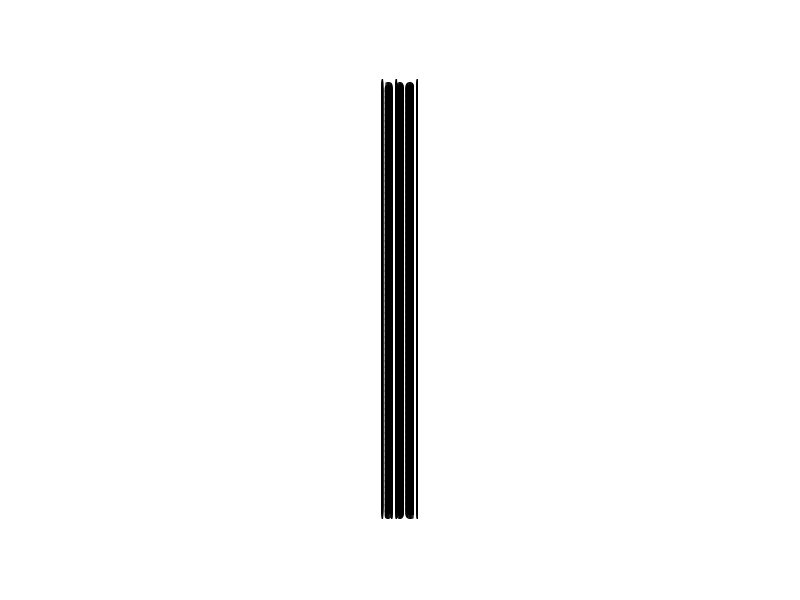
\includegraphics[width=\columnwidth]{testNetworkx500A}
\caption{Arbre linéaire de taille $500$ avec labels obtenu avec NetworkX et Maptplotlib. \label{arbre500NkxA}}
\end{figure}

\begin{figure}[h]
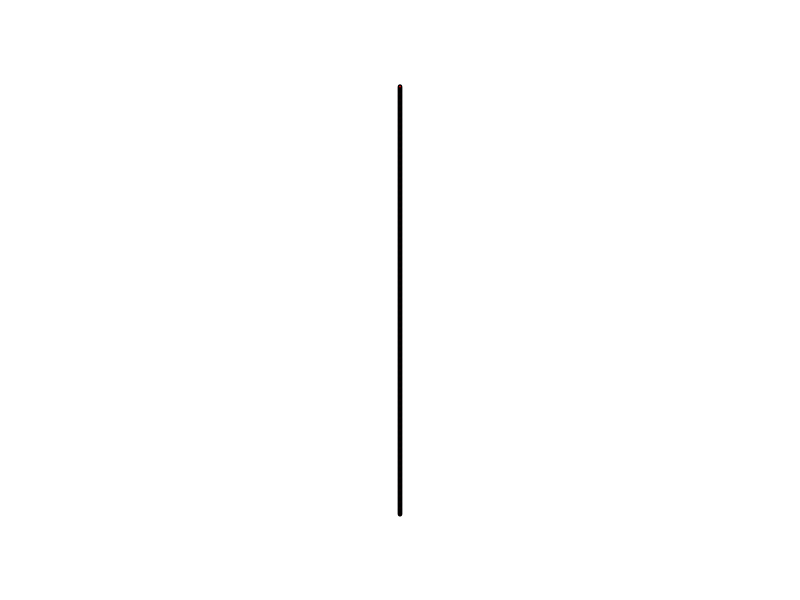
\includegraphics[width=\columnwidth]{testNetworkx500B}
\caption{Arbre linéaire de taille $500$ sans labels obtenu avec NetworkX et Maptplotlib. \label{arbre500NkxB}}
\end{figure}

\begin{figure}[h]
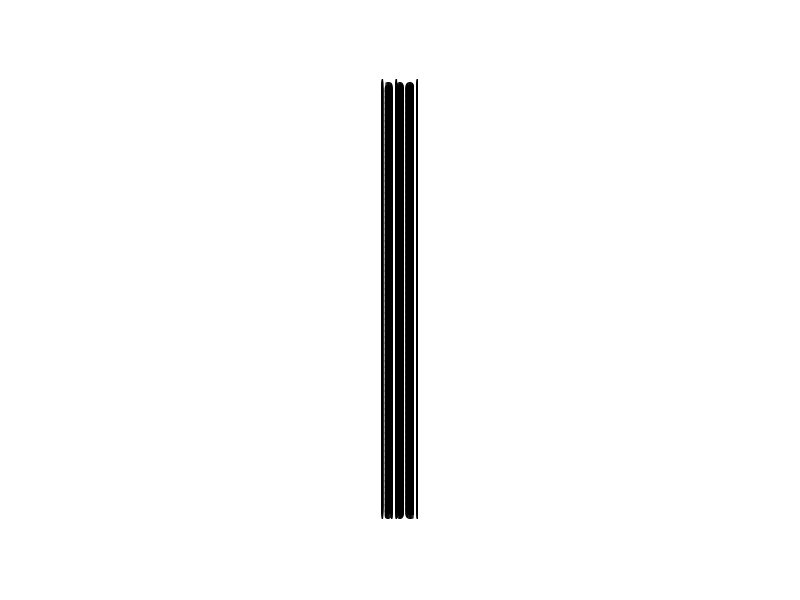
\includegraphics[width=\columnwidth]{testNetworkx500A}
\caption{Arbre linéaire de taille $10000$ avec labels obtenu avec NetworkX et Maptplotlib. \label{arbre10000NkxA}}
\end{figure}

\begin{figure}[h]
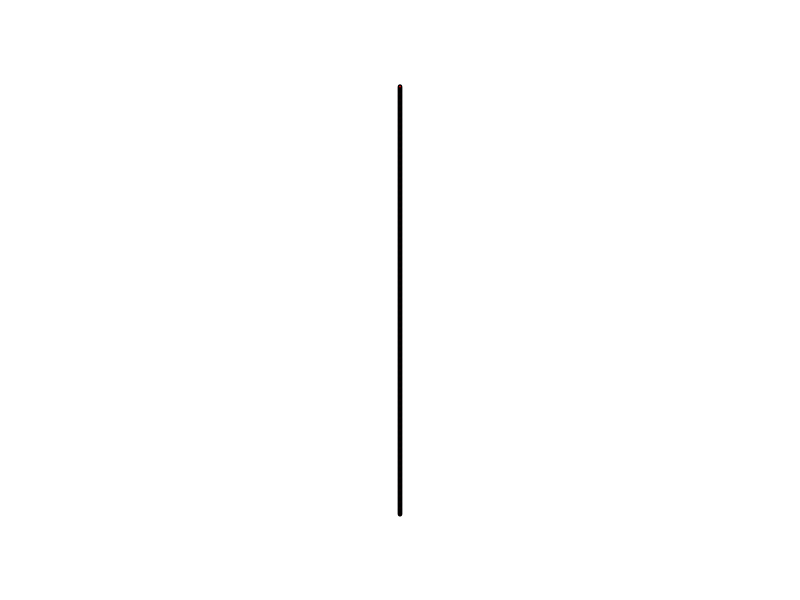
\includegraphics[width=\columnwidth]{testNetworkx500B}
\caption{Arbre linéaire de taille $10000$ sans labels obtenu avec NetworkX et Maptplotlib. \label{arbre10000NkxB}}
\end{figure}
